\documentclass[compexam,copyrightcc]{MSUstyle}
%
%  Created by Seth Humphries 
%  Update and maintained by Prof. Mark Owkes mark.owkes@montana.edu
% 
%%    Copyright (c) 2007-2012 Seth D. Humphries
%%    This work is licensed under the Creative Commons
%%    Attribution-Noncommercial-Share Alike 3.0 License. To view a copy
%%    of this license, visit http://creativecommons.org/licenses/by-nc-sa/3.0/;
%%    or, (b) send a letter to Creative Commons, 171 2nd Street, Suite
%%    300, San Francisco, California, 94105, USA. 
%
%  Version 2.0, check for periodic updates on the bitbucket repository
%
% DEFAULTS --------------------
% The default options are as follows:
%   \documentclass[12pt,letterpaper,oneside,openright,%
%       doublespaced,normalmargins,dissertation,final,numreset]{MSUstyle}
%
% default options do not need to be entered. Defaults will generate a document 
% that conforms to the MSU Electronic Thesis/Dissertation  (ETD) guidelines. 
%
% MASTERS THESIS ---------------
%  use \documentclass[thesis]{MSUstyle} to adjustment the front matter according to ETD style rules that
% are different for a thesis than for a dissertation.
%
% COMPREHENSIVE EXAM -----------
% \use \documenatclass[compexam]{MSUstyle} to format the document for a written
% comprehensive exam. This only changes "dissertation" to "comprehensive exam";
% everything else is the same as the dissertation format. This is an acceptable
% format for the written comprehensive exam in the Electrical and Computer
% Engineering department; other departments may vary.
%
% COPYRIGHT OPTIONS -----------
% If you want to license your work under a Creative Commons BY 4.0 license,
% use the copyrightcc option
%
% ADDITIONAL OPTIONS ----------
% 10pt, singlespaced, and draft allow you to require less number of pages for editing
% A draft version number can be set with, e.g., \draftver{1.0}
%
% numberedsections provides numbered chapter and section titles
%
% appendsingle/appendmultiple is required if you have one/multiple appendices, remove if you do not have an appendix
%
% nonumreset does not add chapter to labels of figures, tables, etc. (not recommended)
%
% PRINTING OPTIONS ------------
% oneside,openright (defaults) 1" margin on all sides of pages (use for electronic documents and submission to grad school)
% oneside,openright,bigmargin larger margin on left side of pages (optionally use for electronic documents and submission to grad school)
% twoside,openany  larger margins alternate left/right sides for binding (use for printing on minimal number of pages)
% twoside,openright larger margins alternate left/right sides for binding and ...
%                               blank pages added so chapter start on right page (use for nicest printed material)

% ========================= %
%  Packages                 %
%  (add as needed)          %
% ========================= %
\usepackage[final]{graphicx} %for the \includegraphics command and figures put [final] before ...
%%    {graphix} if you want figures to show up even while in draft mode
\usepackage{subcaption}    % to be able to have multiple plots in one figure
\usepackage{xcolor} % for changing text color in chapters \textcolor{red}{red text read here}. 
\usepackage[final]{listings} % used for formatting code
\usepackage[pdftex,hidelinks]{hyperref}



% Default to using IEEE-style numeric references. Change as desired
% \usepackage[
% 	backend=biber,
% 	style=numeric,
% 	sorting=none,
% ]{biblatex}

% \addbibresource{misc.bib}


\usepackage{amsmath, amssymb}
\usepackage{lipsum} % Generates random text
%\usepackage{showframe} % View margins

\usepackage{booktabs}

\usepackage[section]{placeins}


\usepackage{breakurl}
\usepackage{dirtytalk}
\usepackage{amsmath,amssymb,amsfonts}
\usepackage{algorithmic}
\usepackage{textcomp}
\usepackage{multirow}
\usepackage{bm}

% Style of code listings (Change as needed)
\lstset{%set Code listings styles
	language=Matlab, % program language for keywords and comments styles
	basicstyle=\small, %font size and style
	identifierstyle=\color{red}, %variable name style
	stringstyle=\ttfamily, %string style
	keywordstyle=\color{blue}\bfseries, %language keyword style
	commentstyle=\color{black}\itshape, %commentstyle
	breaklines=true,  % sets automatic line breaking
	breakatwhitespace=false,   %break line not just at whitespaces
}

\graphicspath{{./figures/}}

% ======================= %
%  User defined commands  %
% ======================= %
\newcommand{\etc}{etc.}
\newcommand{\eg}{e.g.}
\newcommand{\ie}{i.e.} 

\def\x{{\mathbf\ x}}
\def\L{{\cal\ L}}

\DeclareMathOperator*{\argmin}{argmin}
\DeclareMathOperator*{\Proj}{Proj}

% =============================== %
%  Definitions: Change as needed  %
% =============================== %
\name{Kaveen Gayasara Liyanage} %PUT your FULL name here (First Middle Last)
\DocTitle{Sparse Representation Method for Whole Graph Embedding} 
% \OWNwebpage{http://mywebsite.net} %your personal webpage
\degreetitle{Electrical Engineering} % may be different than department... ie MS in Electrical Engineering is not Elect. and Com. Engnr degree.
\department{Electrical and Computer Engineering} 
\committeechair{Dr.\ Bradley Whitaker} 
\departmentchair{Dr.\ Department Chair}
\graduatedean{Dr.\ Graduate Dean}
\submitdate{December 2022} 
\copyrightyear{\the\year} % add one to year if document submitted in Dec.
\draftver{1.0} % versioning for use with draft option

% put searchable words you want internet search engines to find here
\keys{keywords, latex, MSU, Montana State University} 
 
%  Configuration of hyperref package
\hypersetup{%
	% bookmarks=true, %show bookmarks when opening pdf
	bookmarksdepth=3, %show up to subsubsections in pdf bookmarks
	citecolor=black, %citations show up black
	colorlinks=true, %use colored links
	draft=false, % prevents hyperref from draft mode...keeps bookmarks and hyperlinks in draft mode
	filecolor=black, %included file links are black text
	linkcolor=black, %the colored links are black for an ETD but can be otherwise
	pdfauthor={\name}, %pdf document maker is you
	pdfcreator={\name\ by\ PDFLaTex}, %pdf document maker is you
	pdfdisplaydoctitle=true, % make display title the same as the document title instead of the filename
	pdffitwindow=true, %fits one page into the open pdf reader window
	pdfkeywords={\keys}, %searchable keywords
	pdfsubject={\degreetype\ for \name}, %the \  is to give a space
	pdftitle={\DocTitle}, %pdf document title is now ETD title
	plainpages=false, %use hyperlinks in pages, gets rid of a lot of warnings too
	urlcolor=black %website links are black text
}%

% ================================ %
%         Actual Document                                              %
% ================================ %
\begin{document}

% Front matter...before your text
\begin{preliminary}

  % Dedication page (optional, comment out if not using)
%   \begin{dedication} 
%     \input{dedication} 
%   \end{dedication}

  % Acknowledgements page (optional, comment out if not using)
  \begin{acknowledgements}
    Part of the proposal is funded by DHS  
  \end{acknowledgements}

  %vita page (optional, comment out if not using)
%   \begin{vita}
%     \input{vita} 
%   \end{vita}

  % Table of Contents, List of Figures|Tables|etc.
  \contents\
  
  % Nomenclature page (optional, comment out if not using)
%   \begin{nomen}
%     \input{nomenclature} 
%   \end{nomen}


  % Abstract
  \begin{abstract}
    \lipsum[1]
  \end{abstract}
\end{preliminary}

% Dissertation chapters:  add/change as needed
\chapter{Introduction}\label{ch:introduction}

Sparse representation has gained 

Graph representation has gained wide popularity as a data representation method in many applications. Graph embedding methods convert graphs to a vector representation and are an important part of a data processing pipeline. In this paper, we utilize sparse dictionary learning techniques as a graph embedding solution. Sparse representation has notable applications in signal image processing. Inspired by the Graph2Vec algorithm, we aim to modify the Doc2Vec model training portion of the Graph2Vec by incorporating unsupervised dictionary learning. We investigate the viability of using the sparse dictionary learning technique KSVD for graph data. We train the dictionary on Weisfeiler-Lehman graph sub-tree kernel features. Furthermore, we use graph-based labeled data sets to compare classification results with several existing graph embedding methods. Findings show that using the learned sparse coefficients as features for a supervised machine learning algorithm provides on-par classification results when compared to other graph embedding methods. 

Random references\cite{Aharon2006}.

\begin{figure}[b!]
    \centering
    \includegraphics[width=0.8\textwidth]{example-image-duck}
    \caption[Example duck]{Example duck.}\label{fig:example}
\end{figure}
\chapter{Background}\label{ch:Background}

\section{Graphs Embedding}
Graph data is usually highly dimensional and defined in a non-euclidean form. Hence, typical processing methods defined on euclidean spaces cannot be used on graph data. Graph embedding methods convert the graph data into a vector representation while trying to preserve original graph properties\cite{Cai2018}.%\cite{Chen2020, Cai2018}.
Graph embedding methods can be classified as node embedding, edge embedding, hybrid embedding, and whole graph embedding. In literature, a distinction is made between graph representation learning and graph embedding\cite{Cai2018, Chami2022}, where graph representation does not require the final vector to be low-dimensional. In this paper, we focus on whole graph embedding, where each entire graph is represented as a vector\cite{Maddalena2021}. The vector representation can be used to compare graph similarity for important tasks, including classification and clustering. The main challenges in whole graph embedding are how to capture the properties of a whole graph and how to make a trade-off between expressiveness and efficiency\cite{Cai2018}. Several methods have been proposed for whole graph embedding, including matrix factorization, deep learning, edge reconstruction, graph kernel, and generative models\cite{Cai2018, Maddalena2021}.

Graph2Vec is a popular neural network-based architecture for graph embedding\cite{Narayanan2017}. Some advantages of Graph2Vec are that the model is trained in an unsupervised manner, the learned model is task agnostic, the algorithm is data-driven, and resulting vectors capture structural equivalences. Graph2Vec utilizes the non-linear Weisfeiler-Lehman (WL) kernel, %\cite{weisfeiler1968reduction},
which is shown to outperform other linear kernels\cite{shervashidze2011weisfeiler}. %\cite{shervashidze2011weisfeiler, Yanardag2015}.
WL kernel is used to rename the nodes using a hash value that represents a rooted sub-graph on the given node. These sets of node names are viewed as a set of words in a document. The techniques from the Natural language processing (NLP) domain are borrowed for learning an embedding. Doc2Vec is based on Word2Vec\cite{Mikolov2013}, in which a feed-forward neural network (NN) ``SkipGram'' model with negative sampling is used to learn a representation of word sequences\cite{Le2014}. Using the SkipGram model, the nodes with similar neighborhoods are embedded closer together\cite{Rong2014}. The Graph2Vec is implemented in the ``KarateClub'' python package\cite{Karateclub}\footnote{\url{https://karateclub.readthedocs.io/en/latest/}}. An overview of the implementation of the Grap2Vec is shown in Fig.\ref{fig: G2V}, where a vocabulary of sub-tree structures is generated using a WL sub-tree kernel and a Doc2Vec model is trained on the selected vocabulary. 

Some disadvantages of Graph2Vec are the nonlinearity of the learned embedding and the generated sub-tree structures. Due to the nonlinearity, it is difficult to identify which sub-tree structures are contributing to the similarities and differences among graphs. Hence, we propose a linear representation model to replace the Doc2Vec NN architecture. Further, the SkipGram model is capable of embedding only a single node, rather than node combinations. In addition, the SkipGram model considers the neighborhood of the nodes, which depends on an arbitrary node numbering scheme that may not generalize between graphs in a given application.

\begin{figure}[!tbh]
\centerline{\includegraphics[width=0.9\columnwidth]{figures/Graph_embedding/Gaph2Vec.png}}
\caption{Graph2Vec pipeline overview}\label{fig: G2V}
\end{figure}

\section{Sparse Representation and Dictionary Learning}

There has been a growing interest in the search for sparse representations of signals in recent years. In the field of computer vision it can be reasonably assumed that image patches do not populate or sample the whole input domain\cite{Elad2010}. Sparse coding is a representation learning method which aims to find a sparse representation of an  $n$ dimensional input signal $y_i \in \mathbb{R}^n $ in the form of a sparse linear combination, such that the reconstructed data is $\tilde{y_i} = \alpha_{i,1} d_1 + \alpha_{i,2} d_2 + \cdots + \alpha_{i,K} d_K$. Where $\alpha_i \in \mathbb{R}^K$ is the the sparse vector and  $d_i \in \mathbb{R}^n $ are the dictionary elements (atoms) of a Dictionary $\mathbf{D}$. Sparse representation algorithms optimize  (\ref{eq1}) with a $l_0$ regularization term:

\begin{equation}
    \label{eq1}
    \argmin_{D,\alpha}||\mathbf{Y}-\mathbf{D} \mathbf{ \alpha }||_2^2  \;\; s.t.\;\; \forall i, || \alpha_i||_0 \leq S,
\end{equation}

\noindent where $\mathbf{Y}=[y_1,y_2,.., y_N] \in \mathbb{R}^{n\times N}$ denotes the $N$ number of input signals, $ \mathbf{D} = [d_1,d_2,\ldots,d_K] \in \mathbb{R}^{n \times K}$ is the learned dictionary of size $K$, $\mathbf{ \alpha } = [\alpha_1,\alpha_2,\ldots,\alpha_N ] \in \mathbb{R}^{K \times N}$ is the sparse representation of the input signal, and $S$ is the sparsity constraint of $\alpha_i$ (maximum number of non-zero elements). Usually  $K > n$, in which case the dictionary is called over-complete. If $K = n$ the dictionary is called complete and if $K < n$ it is called under-complete.

Equation (\ref{eq1}) can be solved by alternating between the following two stages. First, sparse coding is to calculate $\alpha$ with a fixed over-complete dictionary $D$. Second, dictionary learning is performed to update $D$ with a fixed $\alpha$. K-means Singular Value Decomposition (K-SVD)\cite{Aharon2006, Rubinstein2013} has emerged as an effective and popular algorithm for sparse representation tasks. K-SVD first initializes a random dictionary. It then alternates between the two stages by utilizing Orthogonal Matching Pursuit (OMP)\cite{Pati1993, Davis1997} for the sparse coding and generalized k-means with Singular Value Decomposition (SVD) for the dictionary update. K-SVD efficiently learns an over-complete dictionary and has been effectively utilized for tasks including de-noising, restoration, and classification.

For classification tasks, in order to improve the performance a more discriminatory representation is required. Jiang \textit{et al.}\cite{Jiang2011, Jiang2013} have presented a Label Consistent K-SVD (LC-KSVD) algorithm as an extension of the K-SVD framework, which is a supervised learning algorithm to learn a compact and discriminative dictionary. In LC-KSVD, class-specific dictionary elements are trained separately as an initialization and then combined to learn a discriminative dictionary. A label consistent constraint called \say{discriminative sparse-code error}, reconstruction error and classification error terms are combined to structure a unified objective function to optimize the discriminated dictionary. Due to the class constraints in the sparse coding and dictionary update stages, the input data will forced to be mapped to the dedicated dictionary atoms according to the label information. Consequently in the sparse dictionary domain, a majority of the input signals will be projected to a subspace belonging to a certain class. Hence, a lower order classifier can be trained for the classification. 

Traditional dictionary learning models do not take into account the class imbalances of the training data. Hence the dictionary atoms can be biased towards the larger class. Therefore to address the class imbalances and the structure, a separate dictionary learning algorithm is also employed. Frozen dictionary learning modifies the dictionary learning process as a hierarchical structure to learn a dictionary that can effectively model imbalanced datasets\cite{Carroll2017}. In this algorithm, first, the dictionary learning step is carried out using the K-SVD algorithm on \say{normal} training data. Then the learned dictionary elements are frozen (held constant) and the dictionary is augmented with additional elements by dictionary elements is trained again on abnormalities. This process is repeated for all the remaining classes, by keeping the previously learned dictionaries frozen. The frozen elements of the dictionary represent the \say{normal} aspects of the data, hence the new elements (non-frozen) learn to represent the anomalous aspects of the data that are not present in the \say{normal} data. The frozen dictionary approach could be generally used and applied to the problems including data with or without abnormalities.


\section{Feature Ranking}

eature Ranking (FR) is an essential part of the machine learning pipeline to identify, reduce, remove, or craft features that benefits ML performance and reduce the cost of the operations. In general, FR methods evaluate features by looking at the amount of information they provide and ranking them accordingly so that the most relevant and complementary features can be used in ML training. There are three main categories of methods for FR algorithms: Filter methods (FM), Wrapper methods (WM), and Embedded methods (EM). The FR methods can be further classified as \emph{myopic} and \emph{non-myopic}. Whereas\emph{myopic} methods only evaluate the feature by itself,\emph{non-myopic} methods take into the consideration of interrelationship between the features. Several surveys outline the current state-of-the-art in feature assessment techniques\cite{Uthman2020, Sangodiah2014, Effrosynidis2021, Jovic2015}. A summary of the method's pros and cons are shown in fig.\ref{fig: FR_methods}.

\begin{figure}[!t]
    \centering
    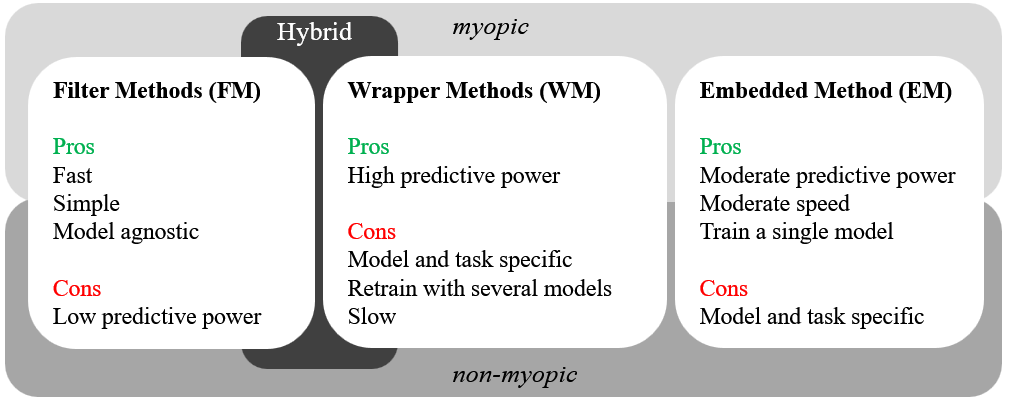
\includegraphics[width=12cm]{figures/eng694/FR_methods.png}
     \caption{Classification of the FR methods and summary of pros and cons}\label{fig: FR_methods}
\end{figure}


In FM, intrinsic properties are evaluated to determine the relevance of the feature. FM methods are generally computationally inexpensive and do not depend on the ML model since the evaluation is done independently. In WM the feature ranking is tied to the ML model performance. This method is more computationally expensive than the FM as it needs to train multiple ML models to identify which features contribute more. WM is model- and task-specific and, as a result, gives better results. However, WM has to be performed again for a different task or a model. EM is similar to WM, however, it performs the feature selection while the ML model is trained. Therefore, time is saved by avoiding training multiple models by sacrificing performance compared to WM\@. EM is also model and task-specific.  

The proposed SR-based methods can be considered as \textit{non-myopic} and a hybrid of FM and EM concepts. To calculate the two metrics, dictionary learning has to be carried out (like EM), which is more computationally expensive than the typical FM\@. However, these metrics do not depend on any ML methods so these FR scores can be used in many applications, unlike EM methods. Furthermore, the proposed metrics do not even have to depend on any particular SR method. However, using a discriminatory dictionary learning and (semi-) supervised SR method would be able to improve the interpretation ability of the data. Since the atoms are a subspace of the original feature space when atoms are learned it takes into account the relationship between all the features hence, these metrics are \textit{non-myopic}. Another main advantage is the ability to decompose the feature importance according to each class with supervised dictionary learning methods. Also, the learned dictionary is not wasted as the dictionary and the calculated sparse coefficients can be used for the training of classifiers in the next stages of the machine learning pipeline. 

Chang and Lin\cite{Chang2008} conducted FR using the weights of the linear SVM\@. Compared with a variant of Fisher-score\cite{Chang2011} (F-score) method, their method showed improved performance. However, it can be only used with a linear SVM\@. Jong, et al.\cite{Jong2004}, proposed an ensemble feature ranking (EFR) algorithm that aggregates results of multiple FR algorithms to gain higher performance. 

Relieff\cite{Kononenko1997} and mRMR\cite{Ding2005} are two commonly used FR algorithms. Both the methods can be considered as \textit{non-myopic} FM algorithms. Zhang et al.\cite{Zhang2019} implemented a novel SR-based feature assessment method called SRDA, where they employ both SR and information theory to identify dependencies and redundancies of the salient features. In this work, they evaluate the learned dictionary atoms (new features) for redundancy and complementary properties. In our work, we try to evaluate the original input features, not the derived sparse features. However, they provide some interesting frameworks for selecting candidate sparse features.

In recent years several deep learning methods have been proposed that achieve high accuracy for data sets. However, deep learning methods lack an intuitive relationship between the learned features and the input layer. Also, they require large computational resources for training and testing. It can be seen that almost all methods that have been used are some form of deep architecture. Usage of deep networks is popular due to the high performance and ability to learn features automatically\cite{Li2019}. We would urge readers to get familiarized with our previous work\cite{Liyanage2020} for a detailed discussion about the advantages of the SR methods concerning deep learning methods.

\section{Hyperbolic Space}

% \chapter{Dictionary Learning on Graph Data with Weisfieler-Lehman sub-tree kernel and KSVD.}\label{ch:graph_sparse}

\section{Introduction}\label{intro}
Graph data is usually highly dimensional and defined in a non-euclidean form. Hence, typical processing methods defined on euclidean spaces cannot be used on graph data. Graph embedding methods convert the graph data into a vector representation while trying to preserve original graph properties\cite{Cai2018}.%\cite{Chen2020, Cai2018}.
Graph embedding methods can be classified as node embedding, edge embedding, hybrid embedding, and whole graph embedding. In literature, a distinction is made between graph representation learning and graph embedding\cite{Cai2018, Chami2022}, where graph representation does not require the final vector to be low-dimensional. In this paper, we focus on whole graph embedding, where each entire graph is represented as a vector\cite{Maddalena2021}. The vector representation can be used to compare graph similarity for important tasks, including classification and clustering. The main challenges in whole graph embedding are how to capture the properties of a whole graph and how to make a trade-off between expressiveness and efficiency\cite{Cai2018}. Several methods have been proposed for whole graph embedding, including matrix factorization, deep learning, edge reconstruction, graph kernel, and generative models\cite{Cai2018, Maddalena2021}.

Graph2Vec is a popular neural network-based architecture for graph embedding\cite{Narayanan2017}. Some advantages of Graph2Vec are that the model is trained in an unsupervised manner, the learned model is task agnostic, the algorithm is data-driven, and resulting vectors capture structural equivalences. Graph2Vec utilizes the non-linear Weisfeiler-Lehman (WL) kernel\cite{weisfeiler1968reduction},
which is shown to outperform other linear kernels\cite{shervashidze2011weisfeiler, Yanardag2015}. WL kernel is used to rename the nodes using a hash value that represents a rooted sub-graph on the given node. These sets of node names are viewed as a set of words in a document. The techniques from the Natural language processing (NLP) domain are borrowed for learning an embedding. Doc2Vec is based on Word2Vec\cite{Mikolov2013}, in which a feed-forward neural network (NN) ``SkipGram'' model with negative sampling is used to learn a representation of word sequences\cite{Le2014}. Using the SkipGram model, the nodes with similar neighborhoods are embedded closer together\cite{Rong2014}. The Graph2Vec is implemented in the ``KarateClub'' python package\cite{Karateclub}\footnote{\url{https://karateclub.readthedocs.io/en/latest/}}. An overview of the implementation of the Grap2Vec is shown in Fig.\ref{fig: G2V}, where a vocabulary of sub-tree structures is generated using a WL sub-tree kernel and a Doc2Vec model is trained on the selected vocabulary. 

Some disadvantages of Graph2Vec are the nonlinearity of the learned embedding and the generated sub-tree structures. Due to the nonlinearity, it is difficult to identify which sub-tree structures are contributing to the similarities and differences among graphs. Hence, we propose a linear representation model to replace the Doc2Vec NN architecture. Further, the SkipGram model is capable of embedding only a single node, rather than node combinations. In addition, the SkipGram model considers the neighborhood of the nodes, which depends on an arbitrary node numbering scheme that may not generalize between graphs in a given application.

\begin{figure}[!t]
\centerline{\includegraphics[width=0.9\columnwidth]{figures/Gaph2Vec.png}}
\caption{Graph2Vec pipeline overview}\label{fig: G2V}
\end{figure}

\begin{figure}[!t]
\centerline{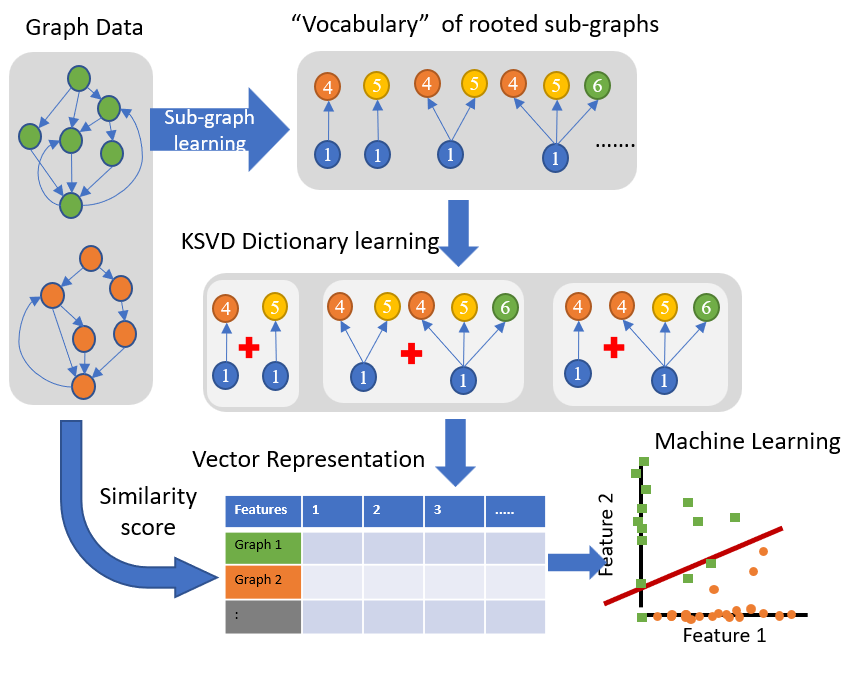
\includegraphics[width=0.9\columnwidth]{figures/GraphKSVD.png}}
\caption{Proposed WL+KSVD pipeline overview}\label{fig: GKSVD}
\end{figure}

Sparse representation is a technique used to learn a dictionary that lies in the original feature domain and calculate a sparse representation using a linear combination of a few dictionary elements (atoms)\cite{Elad2010}. %\cite{Elad2010, Zhang2015}.
The main advantages of using sparse representation are linearity and sparsity: the learned embedding consists of linear combinations of sub-tree structures; sparse representations allow using low-order classifcation models due to the low VC dimension\cite{Neylon2006}. Sparse representation was originally introduced in the signal and image processing domains, however recently it has been utilized in graph-related processes. Several methods have been proposed to represent graph signals on a fixed graph topology with sparse representations with theoretical guarantees\cite{Yankelevsky2019}. %\cite{Subbareddy2019, Thanou2013, Zhang2021, Yankelevsky2020}.
Recent work by Matsuo et al.\cite{Matsuo2019} develops a method to represent different network topologies with sparse representation. However, their work is still limited by requiring graphs to be undirected and requiring all topologies to have the same number of nodes.

To address the shortcomings in sparse vector-based graph representations, we introduce a framework to incorporate WL sub-tree kernel with sparse representation methods specifically aimed at machine learning classification tasks. Our framework allows sparse representation to be applied to graphs with different topologies and different numbers of nodes. In addition, the input graphs can be directed and can incorporate node features. An overview of the proposed WL+KSVD pipeline is shown in Fig.\ref{fig: GKSVD}. The proposed method has the flexibility to swap different dictionary learning and graph kernel methods in the framework. The method is tested against several similar graph embedding methods with benchmark datasets. Finally, the python implementation of the framework and the experiments are currently available on Github\footnote{\url{https://github.com/BMW-lab-MSU/WL-KSVD.git}}.

\begin{figure}[!t]
\centerline{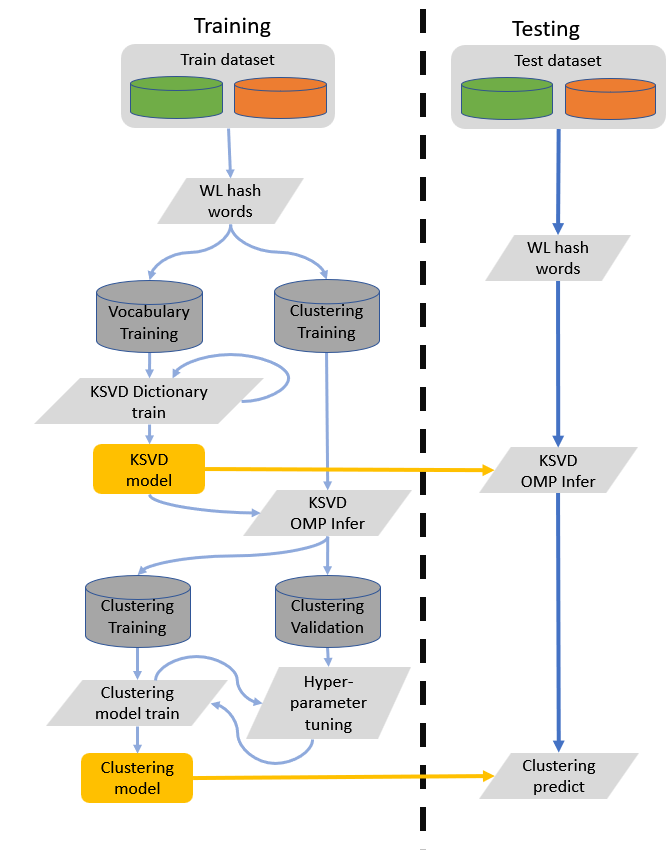
\includegraphics[width=0.9\columnwidth]{figures/Workflow.png}}
\caption{Evaluation Workflow}\label{fig: workflow}
\end{figure}

% \chapter{Dictionary based feature ranking}\label{ch:feature ranking}

\section{Introduction}

Feature Ranking (FR) is an important task used in data science to identify redundant and correlated features. In recent years the increase in data collection availability has led to the curation of high dimensional data sets where the gathered feature may or may not necessarily be sufficient to explain the underlying system. However, in most cases, the collected feature dimensions are redundant or highly correlated. This leads to unnecessary energy and time being wasted in processing, storing, and training models. Training with redundant and correlated features leads to inefficient and over-fitted models that are not robust. Hence identifying which feature dimensions are relevant is vital in developing a more robust machine learning model. Also, understanding which features correspond to which class gives an insight into the model behavior. Then decisions can be made about which features to keep and/or which features to add to explain certain class behaviors. Although many FR algorithms exist, there is no universal method that fits all applications. Each FR method tends to focus on separate aspects of the features depending on the application requirements. Some of these measures are highly nonlinear and complex, and it is hard to have an intuitive understanding of the FR process. Some traditional FR methods do not consider the class distributions or the class imbalances. This unfavorably affects small classes of the dataset as the larger classes will overwhelm the FR metric. Also, most FR methods cannot account for the presence of multiple classes. Although FR algorithms can be applied to each class separately or as a whole, they cannot distinguish feature relevance for each class in the presence of other classes. A discussion about some of the existing popular feature ranking methods is given in section\ref{sec:relatedwork}. 

In this paper, we investigate feature ranking based on Sparse Representation (SR), which has been identified as an effective method to explore internal patterns of data sets\cite{Elad2010}. SR is a method of increasing the dimensions of the dataset so that a better representation of the data can be achieved. This process is linear and easier to understand. The process of SR is divided into two steps. First, it learns a dictionary of subspaces of original feature space. These subspaces or the dictionary elements are called \say{atoms}. Second, it tries to approximately represent each datum as a linear combination of those dictionary atoms. In practice, these two processes are done in an iterative fashion to optimize each other. SR methods are effective under several assumptions. One is the original data can be represented by a subspace of the original feature space. This assumption is valid for many applications, including image and music analysis. The learned atoms reveal some information about the data distribution in the original feature space.

There are two main advantages of incorporating SR for image classification tasks. First, the learned features or dictionary atoms are in the same vector space as the input feature data. Second, representing the data in a sparse domain encourages the use of a linear classifier in the classification stage. Hence, the requirement for computer processing power is less than for deep networks. However, the SR methods for the satellite/airborne image classification are still limited.

We suggest to expand the advantages of SR methods by proposing two novel and simple FR metrics called \textit{dictionary mapping} and \textit{dictionary utilization}. Both can be calculated with any dictionary learning method, including KSVD\cite{Aharon2006}, LC-KSVD\cite{Jiang2011}, and Frozen KSVD\cite{Carroll2017}. We test the metrics using the publicly available Sat-4 and Sat-6 datasets curated by\cite{Basu2015}. Satellite image classification is a challenging problem in the area of land survey and management due to the high variability and associated noise of satellite/airborne imaging. Both data sets comprise manually labeled image patches of 28 $\times$ 28 pixels covering a subset of the continental USA with 1 m$^2$ resolution. Each image contains four color bands: Red (R), Green (G), Blue (B), and  Near Infrared (NIR). Instead of automating the feature learning process, the authors in\cite{Basu2015} and\cite{Liu2020} have selected a set of handcrafted features for the classification task, which has been shown to result in high-accuracy classifiers. We will be utilizing the modified versions of these handcrafted features as the input to our SR methods to learn an over-complete dictionary to calculate sparse coefficients. Previously we have explored the viability of using LC-KSVD with handcrafted features using just the Sat-4 dataset\cite{Liyanage2020}. 

The problem arises as to how the modified handcrafted features affect the overall performance. Hence the proposed metrics were used to rank the importance of the features. For the classification stage, only linear classifiers are utilized to maintain a direct relationship between the classification result and the original input features. The use of linear classifiers allows us to present an analysis of the learned dictionary elements with their relationship to original handcrafted features. Thus, the developed method provides a more intuitive relationship between the learned classifier parameters and the original feature space. The results of the experiments are discussed with limitations and shortcomings in section\ref{sec:conclusion}. 

In this paper, we provide two main contributions. First, we propose two novel FR metrics based on SR methods. Second, we provide feature evaluation examples using Sat-4 and Sat-6 data sets, which will give an idea about how to perform feature evaluation using the proposed metrics. This work is a continuation of our previous work and further details about setup can be found in\cite{Liyanage2020}. 

\section{Related Work}\label{sec:relatedwork}

Feature Ranking (FR) is an essential part of the machine learning pipeline to identify, reduce, remove, or craft features that benefits ML performance and reduce the cost of the operations. In general, FR methods evaluate features by looking at the amount of information they provide and ranking them accordingly so that the most relevant and complementary features can be used in ML training. There are three main categories of methods for FR algorithms: Filter methods (FM), Wrapper methods (WM), and Embedded methods (EM). The FR methods can be further classified as \emph{myopic} and \emph{non-myopic}. Whereas \emph{myopic} methods only evaluate the feature by itself, \emph{non-myopic} methods take into the consideration of interrelationship between the features. Several surveys outline the current state-of-the-art in feature assessment techniques\cite{Uthman2020, Sangodiah2014, Effrosynidis2021, Jovic2015}.

In FM, intrinsic properties are evaluated to determine the relevance of the feature. FM methods are generally computationally inexpensive and do not depend on the ML model since the evaluation is done independently. In WM the feature ranking is tied to the ML model performance. This method is more computationally expensive than the FM as it needs to train multiple ML models to identify which features contribute more. WM is model- and task-specific and, as a result, gives better results. However, WM has to be performed again for a different task or a model. EM is similar to WM, however, it performs the feature selection while the ML model is trained. Therefore, time is saved by avoiding training multiple models by sacrificing performance compared to WM\@. EM is also model and task-specific.  

The proposed SR-based methods can be considered as \textit{non-myopic} and a hybrid of FM and EM concepts. To calculate the two metrics, dictionary learning has to be carried out (like EM), which is more computationally expensive than the typical FM\@. However, these metrics do not depend on any ML methods so these FR scores can be used in many applications, unlike EM methods. Furthermore, the proposed metrics do not even have to depend on any particular SR method. However, using a discriminatory dictionary learning and (semi-) supervised SR method would be able to improve the interpretation ability of the data. Since the atoms are a subspace of the original feature space when atoms are learned it takes into account the relationship between all the features hence, these metrics are \textit{non-myopic}. Another main advantage is the ability to decompose the feature importance according to each class with supervised dictionary learning methods. Also, the learned dictionary is not wasted as the dictionary and the calculated sparse coefficients can be used for the training of classifiers in the next stages of the machine learning pipeline. 

% Chang and Lin \cite{Chang2008} conducted FR using the weights of the linear SVM. Compared with a variant of Fisher-score \cite{Chang2011} (F-score) method, their method showed improved performance. However, it can be only used with a linear SVM. Jong, et al.\cite{Jong2004}, proposed an ensemble feature ranking (EFR) algorithm that aggregates results of multiple FR algorithms to gain higher performance. 

Relieff\cite{Kononenko1997} and mRMR\cite{Ding2005} are two commonly used FR algorithms. Both the methods can be considered as \textit{non-myopic} FM algorithms. Zhang et al.\cite{Zhang2019} implemented a novel SR-based feature assessment method called SRDA, where they employ both SR and information theory to identify dependencies and redundancies of the salient features. In this work, they evaluate the learned dictionary atoms (new features) for redundancy and complementary properties. In our work, we try to evaluate the original input features, not the derived sparse features. However, they provide some interesting frameworks for selecting candidate sparse features.

%In recent years several deep learning methods have been proposed that achieve high accuracy for the Sat-4 and Sat-6 data sets. However, deep learning methods lack an intuitive relationship between the learned features and the input layer. Also, they require large computational resources for training and testing. It can be seen that almost all methods that have been used are some form of deep architecture. Usage of deep networks is popular for satellite/airborne data due to the high performance and ability to learn features automatically \cite{Li2019}. We would urge readers to get familiarized with our previous work\cite{Liyanage2020} for a detailed discussion about the advantages of the SR methods concerning deep learning methods.
 
 SR methods have been previously used for hyperspectral image classification tasks\cite{Dundar2019, Pan2019, Li2018, Huang2017, Tang2014}. However, almost all of them have used pixel-based sparse representation approaches. This approach is not suitable for the Sat-4 and Sat-6 data sets as they do not provide pixel-wise labeling and the patches may contain areas related to other classes. For over-complete dictionary learning, the dictionary dimension is typically around ten times larger than the input dimension. This would be prohibitively large if working directly with the image patches $(28 \times 28 \times 4 \times 10 = 31,360)$. Even though the sparsity is low, the computational cost will be high while manipulating such large data with existing libraries. Hence working with the selected set of meaningful features which should capture the behavior of the images and classes is more suitable. 

\section{Methodology}

\subsection{Feature Extraction}

Rather than extracting features automatically, this paper will follow the works of\cite{Basu2015, Liu2020} and use the same handcrafted 22 features shown in Table\ref{table: Features}, with slight modifications. The RGB value is converted to Hue (H), Saturation (S), and Intensity (I) values, and the color co-occurrence matrix (CCM) is computed\cite{Boyda2017}. Next statistical parameters like mean, variance, 3rd moment, the sum of squares for variance (SSOVH), auto-correlation (AUTOC), and covariance are calculated. The highest Discrete cosine transformation (DCT) frequency value, ignoring the three coefficients that include a DC component, is also used. Several vegetation indexes are computed by utilizing the NIR band information to identify vegetation. The computed features are normalized using the maximum and minimum feature values of the training data with a  buffer of  $5\%$ to allow any variations in the testing data. The data is represented in a logarithmic scale to promote discrimination.
% \begin{table}[tbp]
%     \caption{Handcrafted features for the Sat-4 \& Sat-6 data.}\label{table: Features}
%     \centering
%     \begin{tabular}{|c|c|c|c|}
%         \hline
%         \textbf{} & \textbf{Indices} & \textbf{} & \textbf{Indices}\\
%         \hline
%         1 & I CCM mean & 12 & I std \\
%         \hline
%         2 & H CCM sosvh & 13 & H std \\
%         \hline
%         3 & H CCM autoc & 14 & H mean \\
%         \hline
%         4 & S CCM mean & 15 & I mean \\
%         \hline
%         5 & H CCM mean & 16 & S mean \\
%         \hline
%         6 & Simple Ratio & 17 & I CCM covariance \\
%         & (SR) mean & & \\
%         \hline
%         7 & S CCM 3rd moment & 18 & NIR mean \\
%         \hline
%         8 & I CCM 3rd moment & 19 & Atmospherically Resistant  \\
%         & & & Vegetation Index (ARVI) mean\\
%         \hline
%         9 & I 3rd moment & 20 & Normalized Vegetation Index \\
%         & & & (NDVI) mean\\
%         \hline
%         10 & I variance & 21 & DCT highest non-DC component\\
%         \hline
%         11 & NIR std & 22 & Enhanced Vegetation Index \\
%         & & &EVI mean\\
%         \hline
%     \end{tabular}
% \end{table}

\subsection{Feature Ranking Metrics Based on Sparse Representations}\label{ssec:FR_metric}





%%%%%%%%%%%%%%%%%%%%%%%%%%%%%%%%%%%%%%%%%%%%%%%%%%%%%%%%%%%%%%%
%%%%%%%%%%% Figures placed here for formatting %%%%%%%%%%%%%%%%
%%%%%%%%%%%%%%%%%%%%%%%%%%%%%%%%%%%%%%%%%%%%%%%%%%%%%%%%%%%%%%%
\begin{figure*}[!t]%
\centering
\subfloat[][]{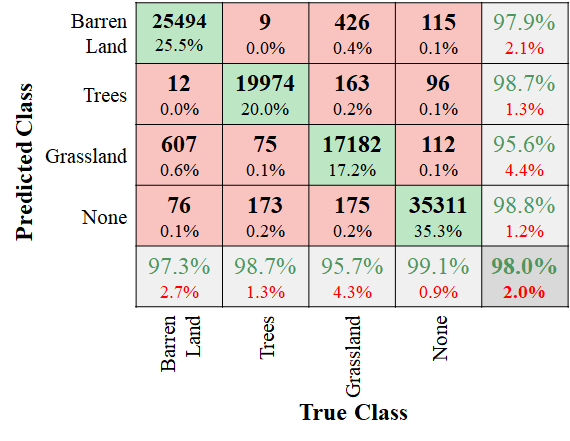
\includegraphics[width=0.6\columnwidth]{S4_FZN.png}}%
\qquad
\subfloat[][]{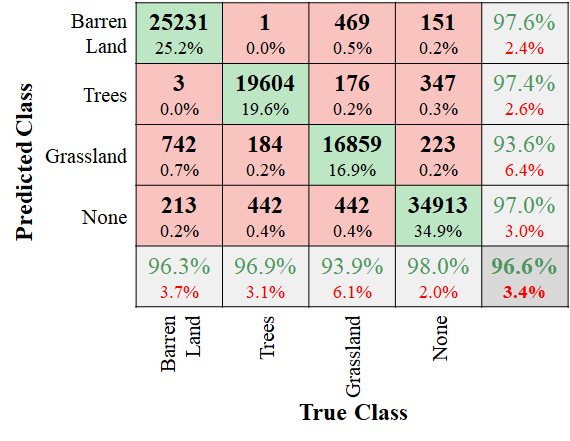
\includegraphics[width=0.6\columnwidth]{S4_LCK.png}}\\
\caption{Confusion matrix for Sat-4 dataset with (a) Frozen (b) LC-KSVD dictionary learning methods.}\label{fig: sat4_rslt}%

%\ContinuedFloat

\subfloat[][]{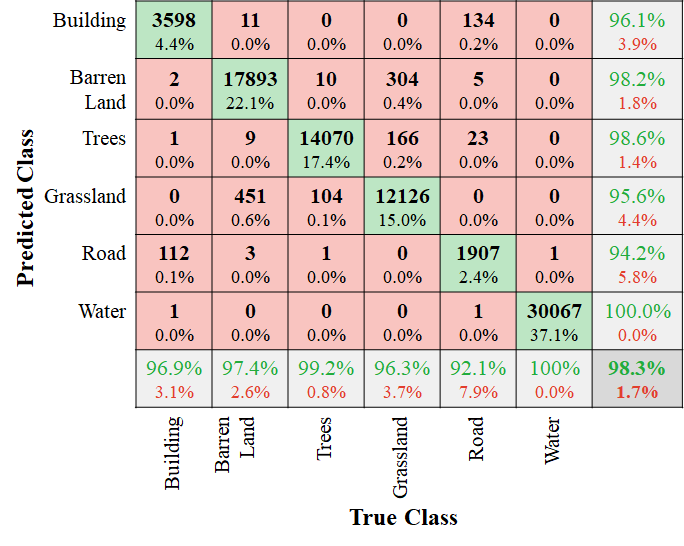
\includegraphics[width=0.8\columnwidth]{S6_FZN.png}}%
\qquad
\subfloat[][]{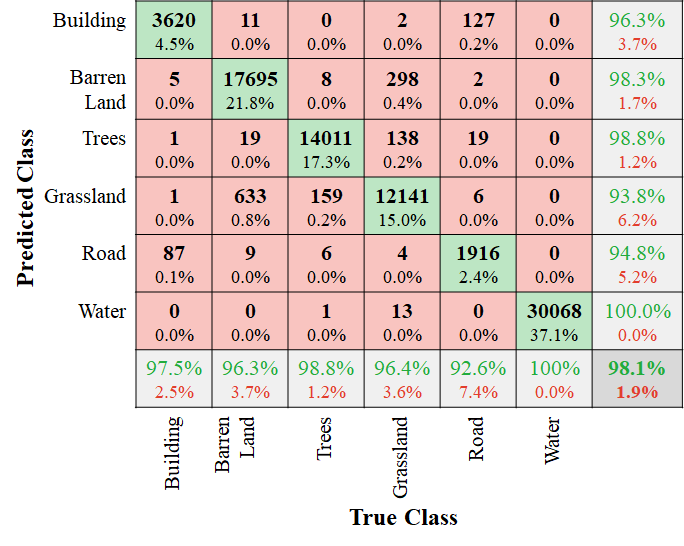
\includegraphics[width=0.8\columnwidth]{S6_LCK.png}}
\caption[]{Confusion matrix for the Sat-4 (a,b) and Sat-6 (c,d) datasets with Frozen (a,c) and LC-KSVD (b,d) dictionary learning methods.}%
\label{fig: sat6_rslt}%
\end{figure*}
%%%%%%%%%%%%%%%%%%%%%%%%%%%%%%%%%%%%%%%%%%%%%%%%%%%%%%%%%%%%%%%
%%%%%%%%%%%%%%%%%%%%%%%%%%%%%%%%%%%%%%%%%%%%%%%%%%%%%%%%%%%%%%%

Let $\mathbf{F} = [F_1$, $F_2$, $\dots F_d]$ be a set of $d$ features $F$ which are collected or curated. The goal is to rank the feature set $\mathbf{F}$ by evaluating a mean-removed training set of $n$ samples: $\mathbf{\bar{X}} = [x_1, x_2, \dots, x_n] \in \mathbb{R}^{d \times n}$. The set of $k$ classes is defined as $\mathbf{C} = [C_1$, $C_2$, $\dots, C_k]$, where each of the $x$ samples is assigned to a class $C$. In sparse representation the input sample is represented as a linear combination of dictionary elements $D$ in a over-complete ($d \ll m$) dictionary $\mathbf{D} = [D_1, D_2, \dots, D_m] \in \mathbb{R}^{d \times m}$, where the number of dictionary elements used, $s$, is far less than the number of dictionary atoms: $s \ll m$. The set coefficients $\bm{\alpha} = [\alpha_1, \alpha_2, \dots, \alpha_n] \in \mathbb{R}^{m \times n}$ of the linear combination is called the sparse coefficients. Each coefficient vector contains $s$ nonzero entries; the remaining $m-s$ entries are exactly zero. The general objective function used for calculating the sparse representation is given by (\ref{eq:sparse}) with an $\ell_0$ constraint on sparsity.

\begin{equation}
    \label{eq:sparse}
    \argmin_{\mathbf{D},\bm{\alpha}} ||\mathbf{\bar{X}}- \mathbf{D}\bm{\alpha}||_F + ||\bm{\alpha}||_0
\end{equation}

The KSVD algorithm is an efficient iterative method that solves the objective function by, first fixing the $\mathbf{D}$ and optimizing the $\bm{\alpha}$ using orthogonal matching pursuit (OMP)\cite{Pati1993}. Second, it fixes $\bm{\alpha}$ then optimize $\mathbf{D}$ with generalized K-means and singular value decomposition (SVD). Since the learned dictionary is over-complete, the spread of the dictionary atoms can give an insight into which features are more relevant for the representation. Hence, we will be defining simple metrics that will quantify the spread of the dictionary elements in each of the features. First \textit{Dictionary mapping}, $\mathbf{D}_\textrm{map} \in \mathbb{R}^{1 \times d}$, which calculates the sum of the squares of the projections of the dictionary atoms for each feature as given in (\ref{eq:dict_map}), where $\Proj_j$ is the projection operator into feature $F_j$. 

\begin{equation}
    \label{eq:dict_map}
    \mathbf{D}_\textrm{map}(j)= {\sum_{i=1}}^m {\Proj_j(D_i)}^2  = \sum_{i=1}^m \mathbf{D}_{(j,i)}^2 
\end{equation}

 The second metric is the \textit{Dictionary utilization}, $\mathbf{D}_\textrm{util} \in \mathbb{R}^{1 \times d}$, which calculated the utilization of the dictionary elements by the sparse coefficients. This acts as a weighted measure of the \textit{dictionary mapping}. Finally, the weighted dictionary atoms are projected back to original features. The equation is given in (\ref{eq:dict_util}).
 
 \begin{equation}
    \label{eq:dict_util}
    \mathbf{D}_\textrm{util}(j)= \sum_{i=1}^m \Proj_j(D_i \cdot \sum_{k=1}^n |\alpha_{j,k}|)  
\end{equation}
 
The KSVD algorithm learns the dictionary in an unsupervised manner, hence we cannot get dictionary elements that are optimized for class discrimination. Therefore several other methods have been proposed to learn a more discriminative dictionary by learning in a supervised manner, giving us a strong association of dictionary atoms with each class. Here we will be exploring two such methods, LC-KSVD and Frozen KSVD\@. By doing so we can decompose the proposed metrics into classes, which gives more insight into feature behavior concerning class labels. In LC-KSVD the algorithm enforces two extra constraint terms related to dictionary association with each class and linear classifier performance. Hence, samples are forced to utilize a subset of the dictionary atoms for their representation leading to a more discriminatory dictionary. However, when imbalanced data is presented the LC-KSVD algorithm does not change the dictionary atom distribution. Therefore, Frozen KSVD is proposed to take class imbalances into consideration of dictionary learning. It first learns a dictionary only considering the largest class. Then next largest class is trained with added dictionary atoms while keeping the previously learned dictionary atoms fixed (frozen). This forces the algorithm to learn new dictionary atoms which are associated with only the new class. This is repeated for all the classes such that the added number of dictionary atoms and the sparsity of each class are reduced depending on the class size. 

\section{Results}

\subsection{Classification Accuracy}

We first tested the classification accuracy of using both Frozen KSVD and LC-KSVD followed by linear classifiers. Both methods result in accuracy greater than $96\%$ on the Sat-4 dataset and greater than 98\% on the Sat-6 dataset. The confusion matrices for the two methods for each dataset are shown in Fig.\ref{fig: sat6_rslt}, respectively. For Sat-4  we see a higher confusion between the barren land and grassland. This might be due to the images containing both grass patches and barren land. Future work could mitigate this error by introducing an additional handcrafted feature that could distinguish between the grass and barren land. For the Sat-6, we observe that the water is almost perfectly classified using both methods. Still, the confusion between the barren land and grassland prevails. Also, confusion between roads and buildings is present. This might be caused by a similar composition and color of images in both classes. This could be mitigated by introducing a cost matrix in the classifier training stage to give a higher penalty for \textit{road}-\textit{building} misclassifications. 

Although the accuracy of the proposed method does not meet the state-of-art performances\cite{Liyanage2020}, it does provide other benefits which deep networks lack. First, the usage of simpler linear classifiers reduces the computational complexity and overall training time in the classification stage. Second, since the input features and the learned dictionary elements are in the same space, they provide a more intuitive understanding of the workings of the architecture. By analyzing the dictionary elements that are used in the representation for each class we can understand the impact of each handcrafted feature in the final performance. By doing so, decisions can be made regarding the effectiveness of selected features and whether redundant features are present or additional features are required for specific class separations. This kind of intuitive \say{backward analysis} is not possible with deep networks due to the highly non-linear, interconnected relationship of the network connections between layers. 

\subsection{Dictionary Elements Analysis}

% \begin{figure*}[!t]%
% \centering
% \subfloat[][]{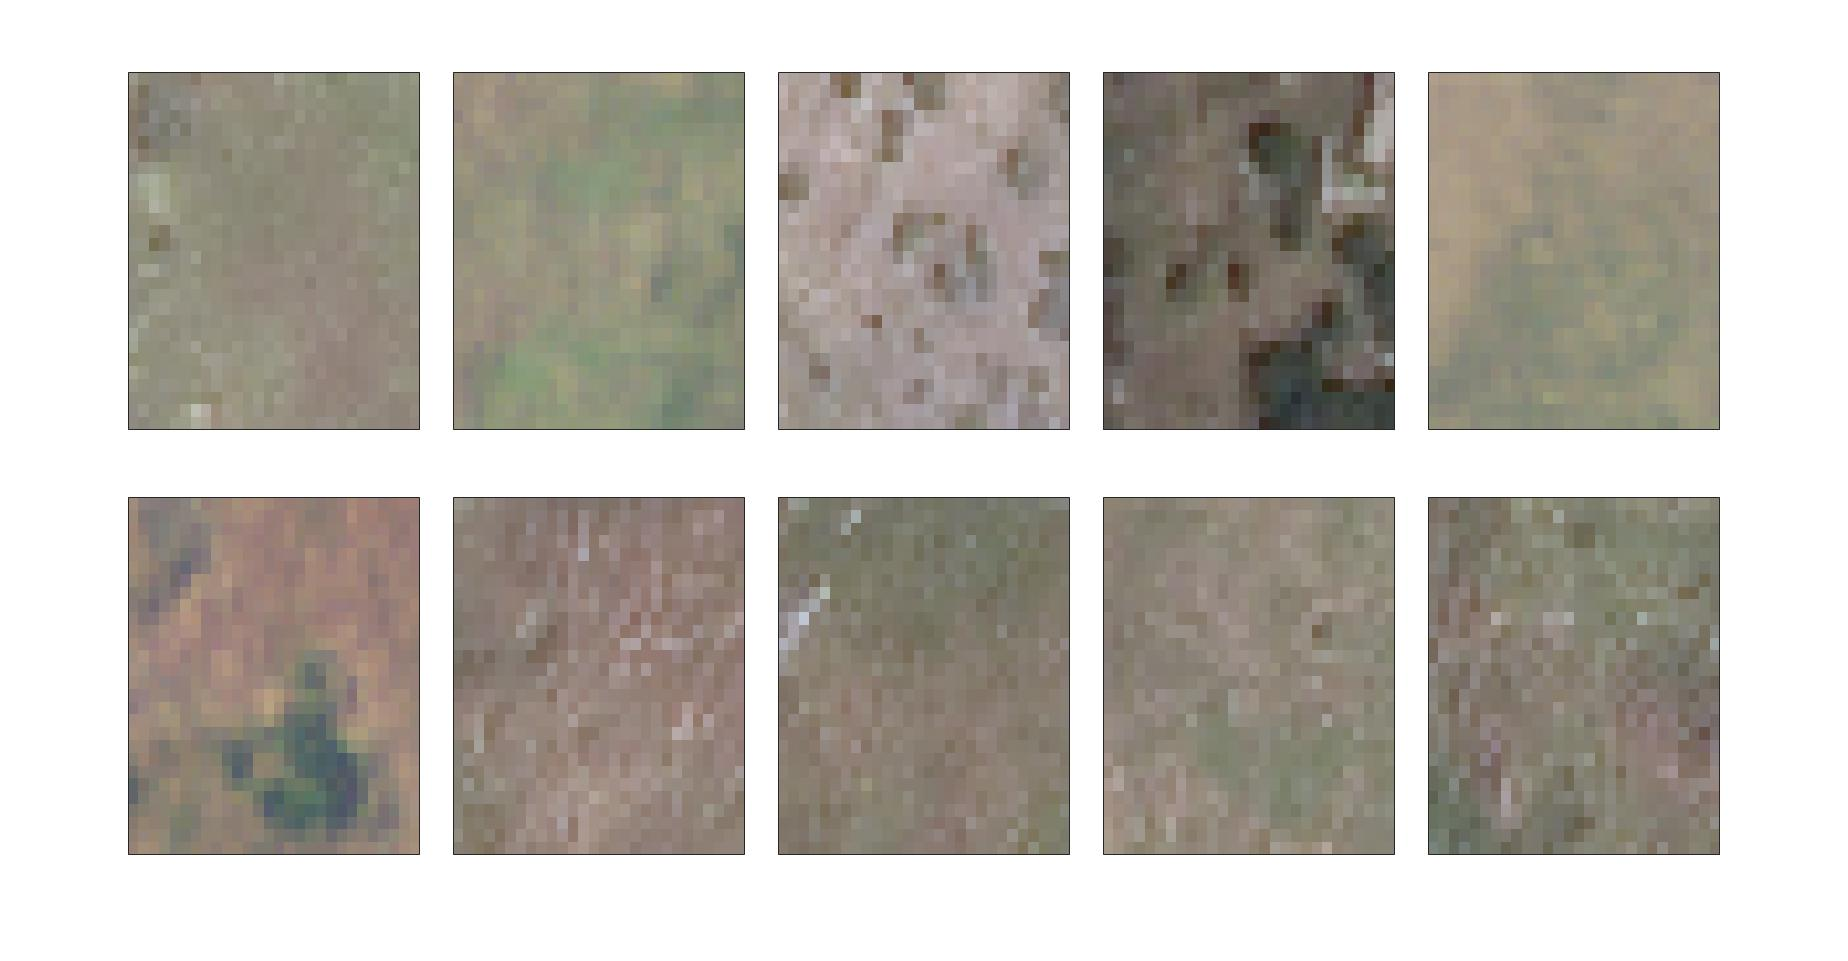
\includegraphics[width=2in]{BL_as_GL.jpg}}%
% \qquad
% \subfloat[][]{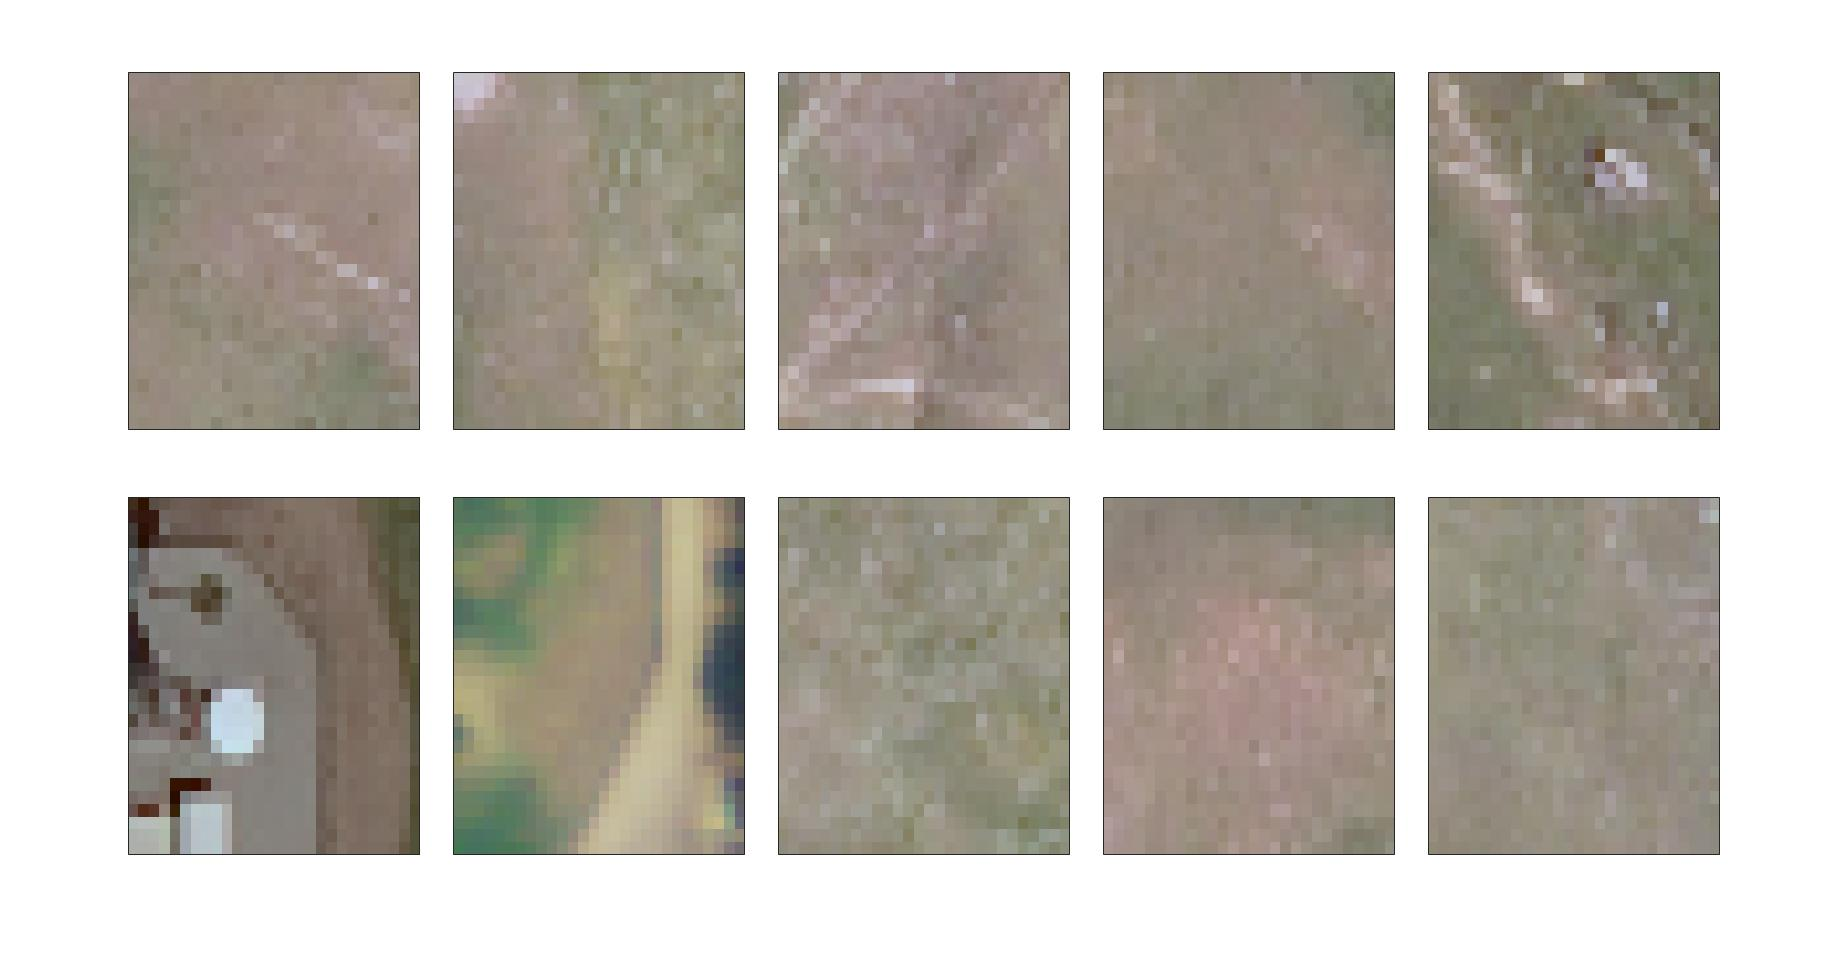
\includegraphics[width=2in]{GL_as_BL.jpg}}
% \caption{Example images with ground truth labels of (a) \textit{barrenland} and (b) \textit{grassland} which are mis-classified as each other.}%
% \label{fig: BL_GL}%
% \end{figure*}

\begin{figure*}[!t]%
\centering
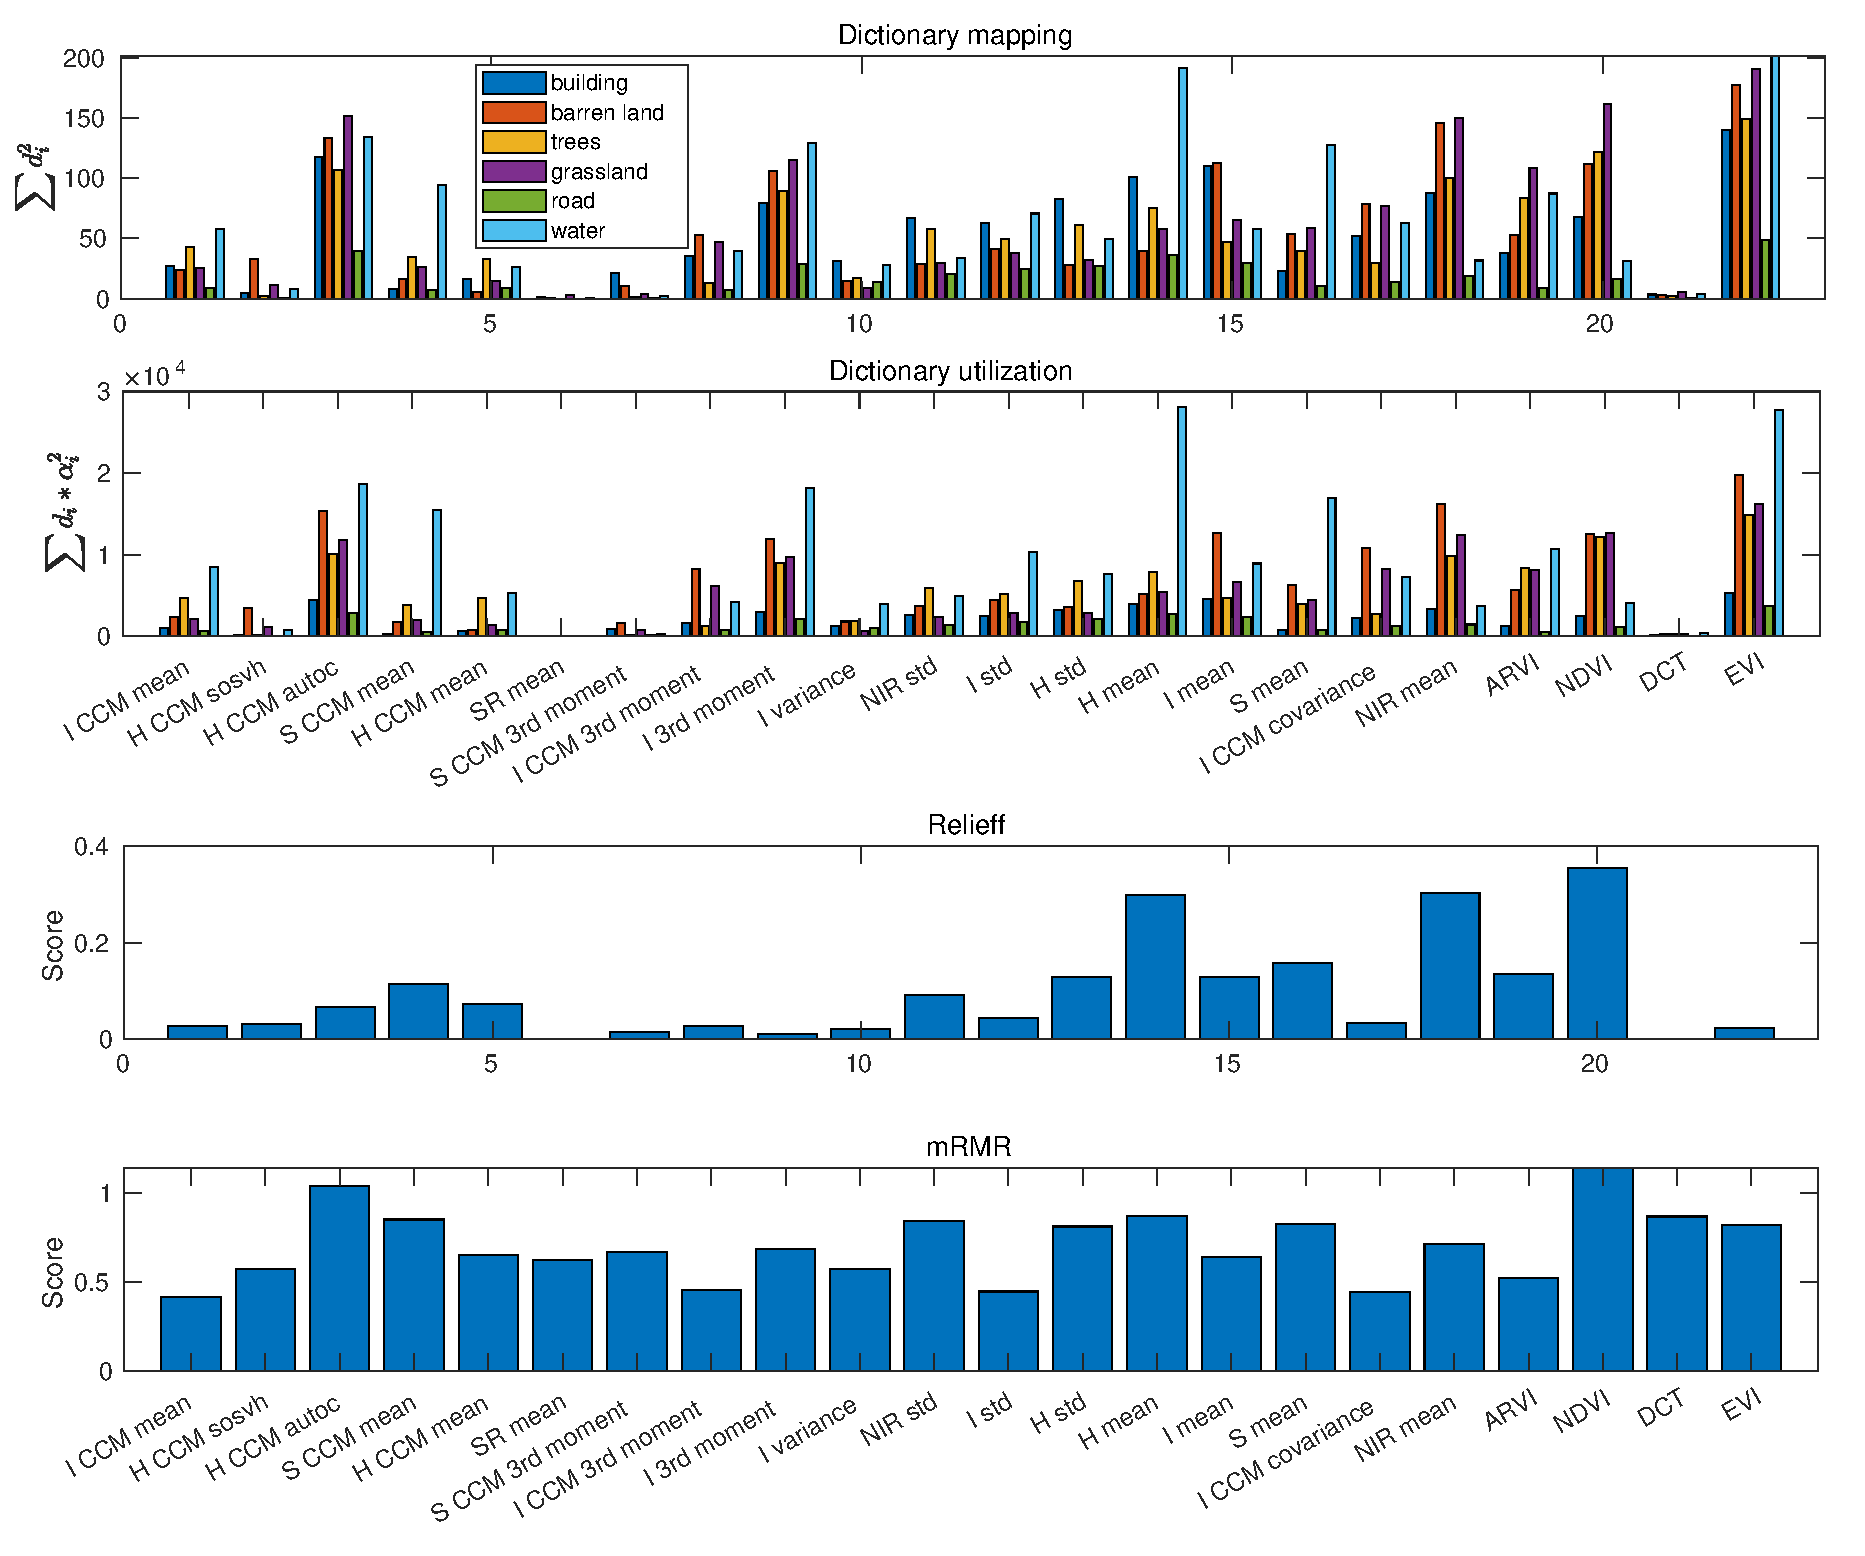
\includegraphics[width=6.6in]{Dict_FR.eps}
\caption{FR scores obtained using various methods on the Sat-6 dataset. The dictionary scores were obtained using frozen KSVD sparse representation.}%
\label{fig:FR}%
\end{figure*}


% \begin{figure*}[!t]
% \centering
% \subfloat[][]{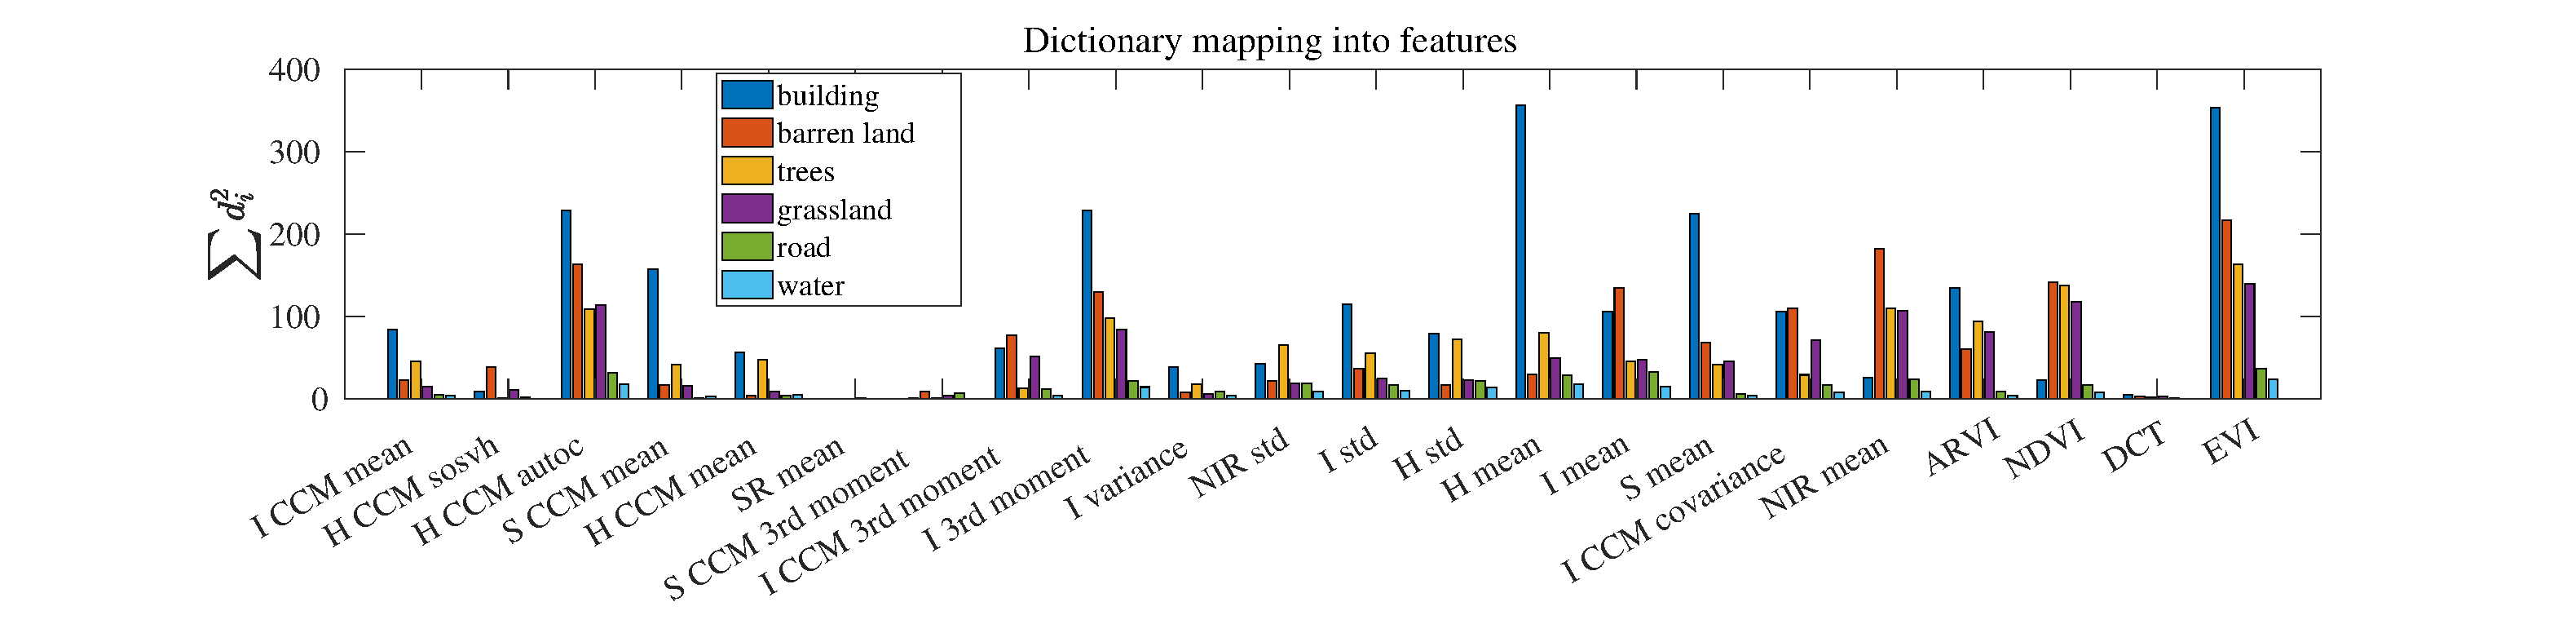
\includegraphics[width=7.2in]{Dict_map.eps}}\label{fig:dict_map}\\ 
% \subfloat[][]{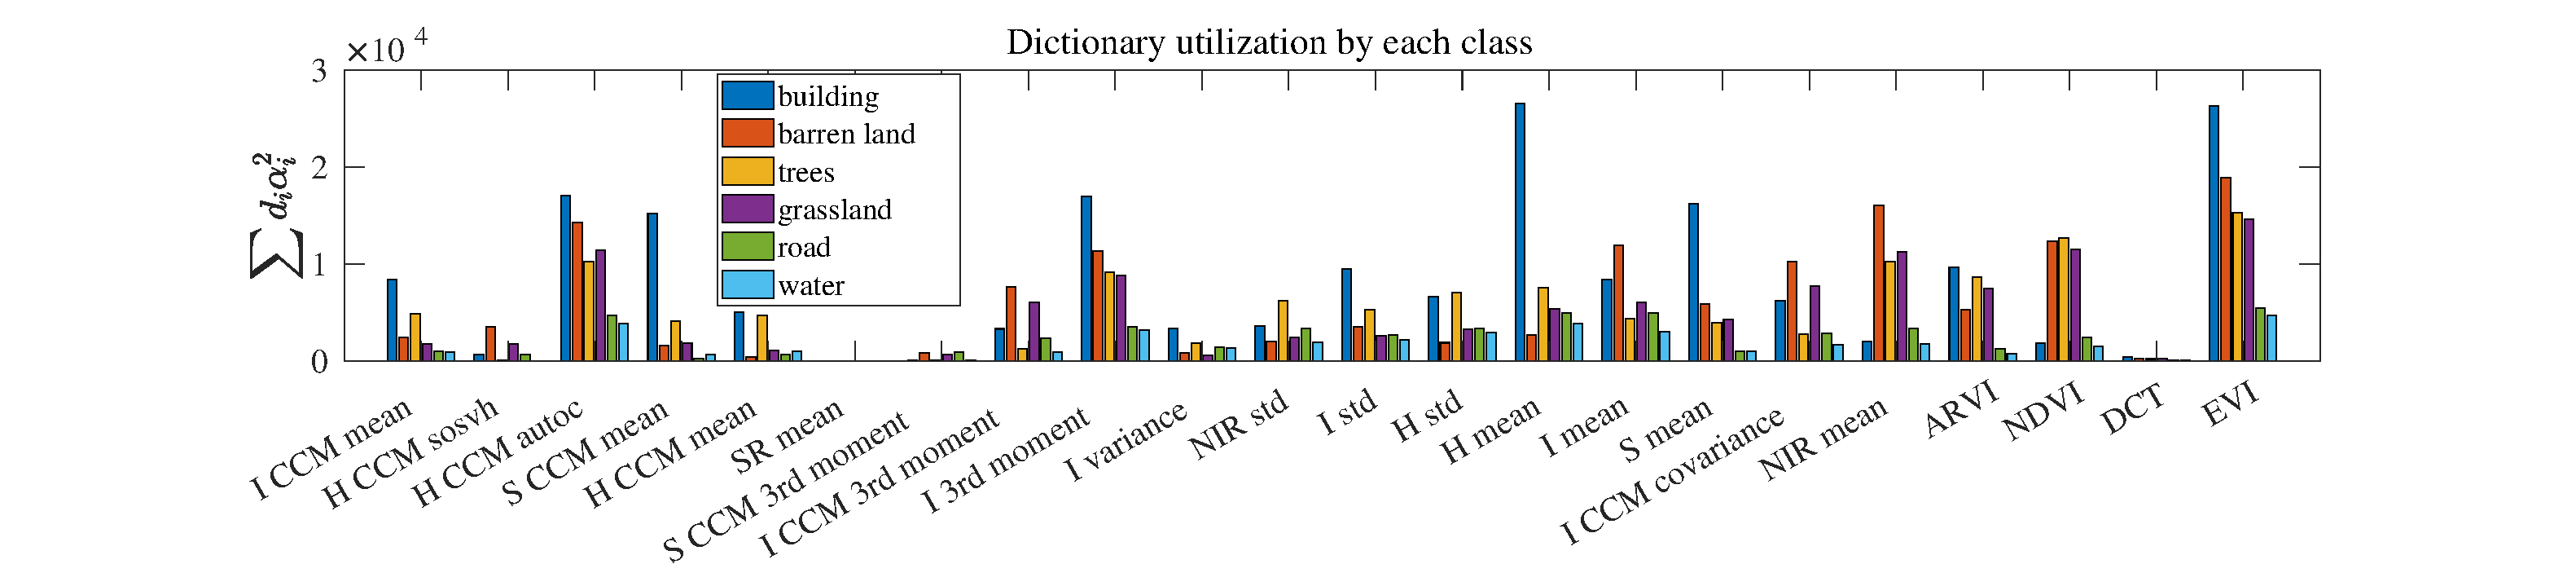
\includegraphics[width=7.2in]{Dict_util.eps}}\label{fig:dict_util}\\ 
% \subfloat[][]{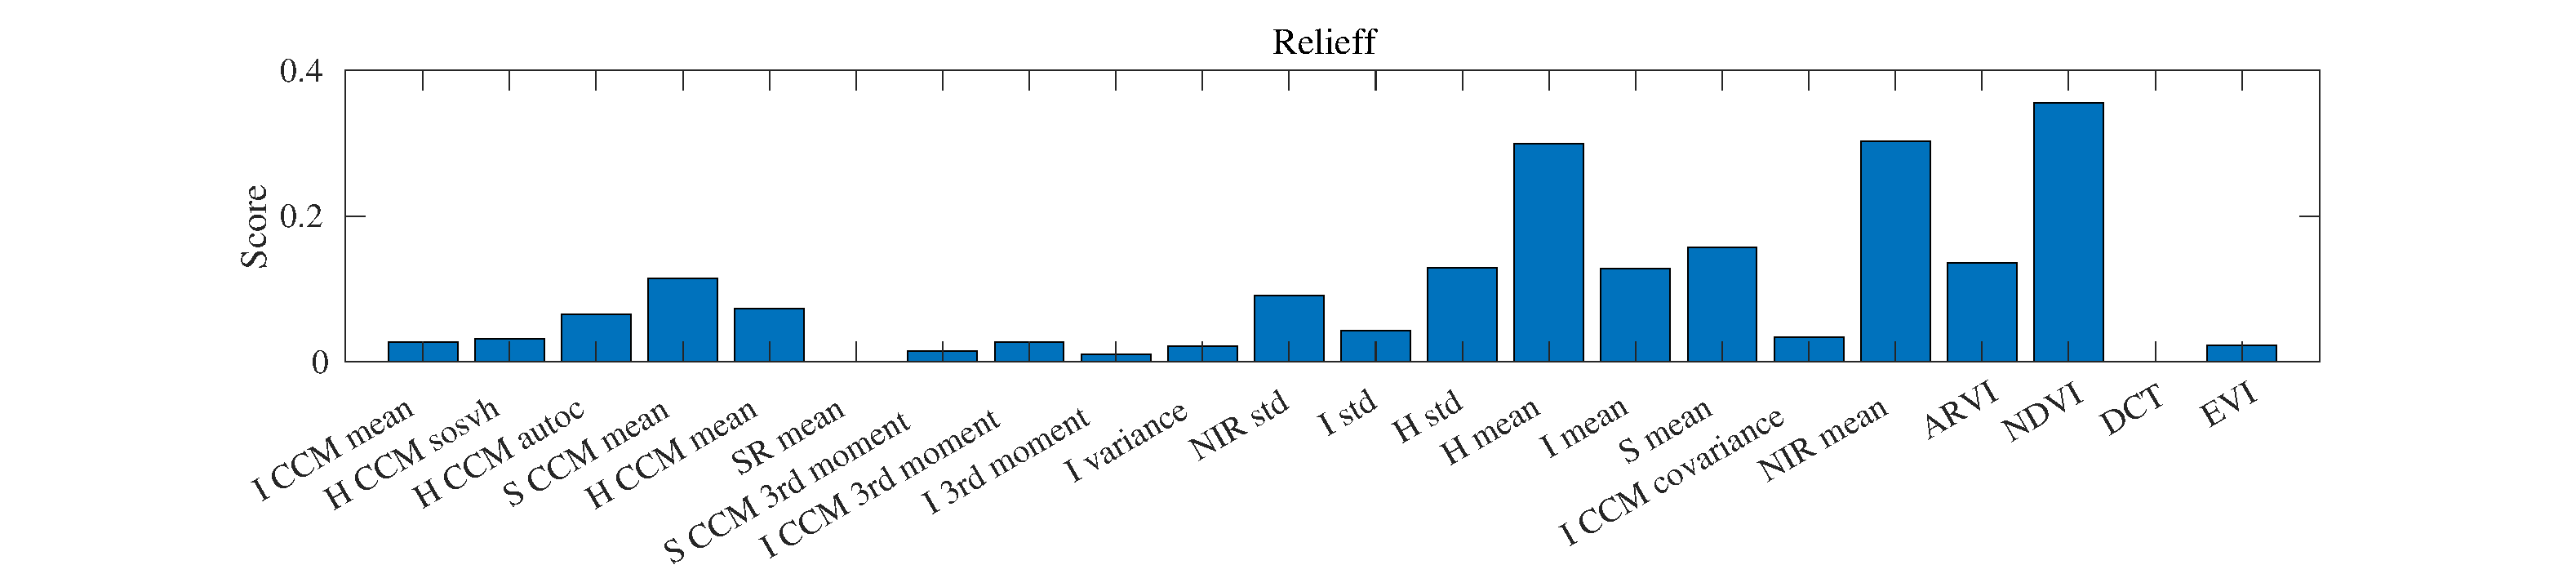
\includegraphics[width=7.2in]{Sat6_Releiff.eps}} \label{relieff}\\
% \subfloat[][]{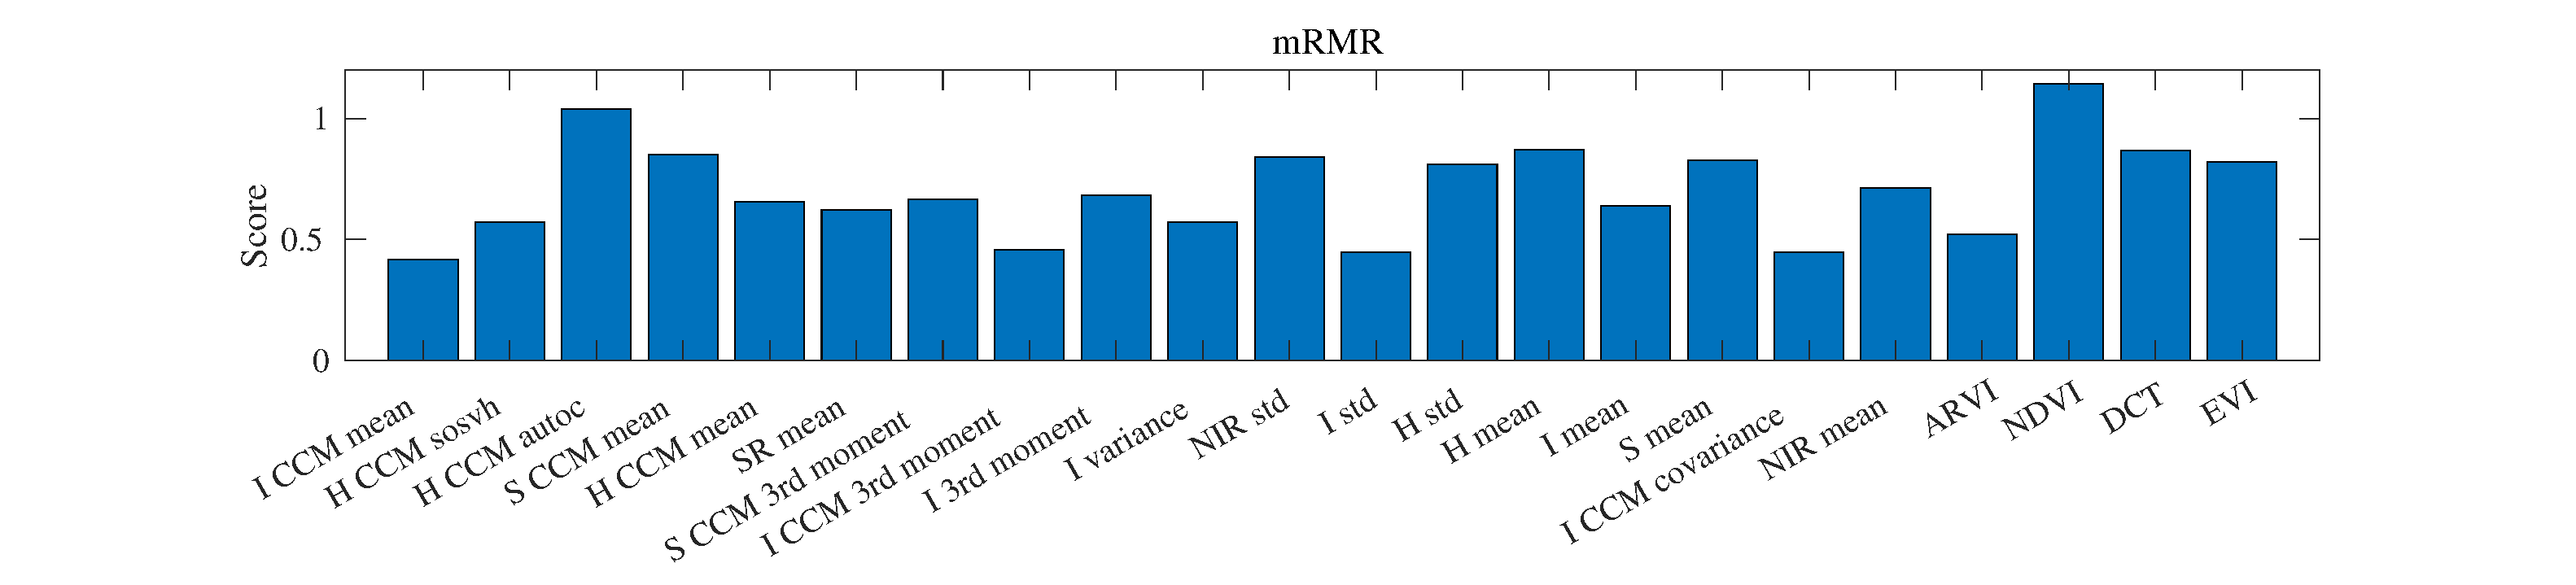
\includegraphics[width=7.2in]{Sat6_mRMR.eps}}\label{fig:mrmr}%
% \caption{Feature utilization by dictionary elements by class}%
% \label{fig:FR}%
% \end{figure*}

When we examine the dictionary atoms used by correctly and incorrectly classified images it can be observed that incorrectly classified images share some of the dictionary atoms that are mostly allocated to the other class. When we transform these dictionary elements back to the feature space we can identify the features that give similar parameters to the two classes, indicating that these features are not able to distinguish between the two classes. Hence, we can decide whether to replace the features or add new features that are capable of separating the two classes. Since our feature domain is considerably small this will not drastically increase the computational burden of the system for this example. This ability to identify the features responsible for misclassifications is not intuitively simple with deep networks and other FR methods. 

As an example, we can take a closer look at the most prevailing confusion between classes \textit{barren land} and \textit{grassland} in the Sat-6 dataset from the Frozen dictionary model. Most of the the misclassified images belonging to these classes contain soil and grass patches. For brevity, we do not present images of the misclassified data points, but the difficulty in producing accurate ground-truth labels likely contributes to the confusion and lower accuracy. This can be observed also in the misclassified \textit{building} class, where many of the images misclassified as \textit{roads} were parking lots. This, combined with the fact that \textit{roads} have very small training data, would accumulate to the low performance of the \textit{road} class. While a similar analysis could be done for images classified with a deep network, the linearity employed by dictionary learning and classification in this work allows for a more comprehensive analysis. 

Fig.\ref{fig:FR} shows the \textit{dictionary mapping} and the \textit{dictionary utilization} of the sparse coefficients used by dictionary elements projected into the original feature space from the frozen KSVD method on Sat-6 data. Since each dictionary atom is associated with a class, the class-wise metric analysis is performed on the original features. It also shows the FR done by the non-class specific Releiff and mRMR methods. Both proposed metrics perform in a similar fashion. While their scores are closer to the Relieff method they are also able to capture some important features predicted by mRMR method (e.g. \textit{H CCM autoc} and \textit{EVI}). The proposed methods also match the Relieff method in identifying SR mean and DCT as underutilized features.

The shortcomings of SR are well recorded in cases where an abundance of bare soil is present, and indices like Soil Adjusted Vegetation Indexes (SAVI) can be used to mitigate this problem\cite{Huete1988}. Due to the presence of similar texture in both \textit{barren land} and \textit{grassland} classes, its DCT components also give similar results. Since we have used a modified and more statistical version of the 22 features selected by\cite{Basu2015}, some features do not perform well with the sparse model. Using sparse coding and linear classifiers, we can identify, evaluate, and improve the necessary input features that might increase the performance of the classification.

Concerning classification performance between the two SR methods used, Frozen KSVD performs slightly better than the LC-KSVD in the Sat-6 dataset. This is possibly due to the strategy Frozen KSVD employs in taking class sizes into account and learning dictionary elements hierarchically. This enables the algorithm to produce dictionary atoms that specifically model the smaller classes. For the Sat-4 dataset, Frozen KSVD performs notably better than LC-KSVD\@. This may be due to the high variability of the \textit{none} class.

\section{Conclusion}\label{sec:conclusion}

In this paper, we have proposed two metrics for feature ranking. Said metrics were compared with some popular FR methods to demonstrate that the ranking yields similar results. These metrics are ML model-independent and can thus be used with a wide variety of classifier models. Additionally, with the class decomposition of the metrics, a better insight can be gained into the model behavior. As a preliminary demonstration, metrics were used with satellite/ airborne scene classification using a sparse representation-based method with the use of linear classifiers. Two discriminative dictionary learning methods, Frozen KSVD and LC-KSVD were tested. We were able to achieve relatively high-end results using an ensemble of simple linear classifiers. The main advantage of utilizing these methods is the ability to gain an intuitive understanding of the relationship between the learned sparse coefficients and the original feature space. We have shown with an example analyses the backward interpretation of the learned sparse coefficients and the classifier to the original feature space which enable an intuitive analysis of the model. 

However, the applications of this method are still not verified to be robust. Several assumptions may have to ascertain to guarantee good performance. The original data itself has to be sparsely structured: it is regarded true for data sets like images, video, and music. Further when the data is high dimensional and has a small number of samples, calculating an over-complete dictionary may not be practical. Using an under-complete dictionary might be an option that is similar to other FR methods. These metrics depend on the original data range and are sensitive to operations like normalization, shrinkage, and mapping. Hence a more robust metric has to be defined to reduce the sensitivity. Also, these metrics cannot be used with non-numeric and discrete features. Hence they have to be omitted from the feature pool to be ranked. In the future, we hope to address some of the above concerns and conduct a thorough experimental verification of the robustness of the metrics. Further analysis will be conducted with relation to other FR algorithms to understand the theoretical relationship.






% REFERENCES
% TODO: "REFERENCES" shows up in all caps in the pdf bookmarks, whereas when using bibtex that was not the case. Other than that, it looks like the formatting is okay when using biblatex instead of bibtex...
% \printbibliography[heading=bibintoc, title={REFERENCES}]
\bibliographystyle{ieeetr}
\bibliography{misc.bib}


% APPENDIX
% If you have an appendix use either the option appendsingle (1 appendix) or appendmultiple (>1 appendix) in your document class
% If you do not have an appendix comment out below and remove the appendsingle/multiple option from the document class
% \appendix
% \include{appendixa}
%\include{appendixb}

\end{document}
% do not put anything after this

